\section{Results}

\subsection{A data-constrained V1 circuit and the mouse reference}
Each network had 1{,}000 fitted GFR cells wired with measured cell-type connection probabilities.
It was driven by an LGN front end and trained with a cell-local e-prop rule (with or without the
spike-history term $\beta$) or with exact BPTT, with the same optimizer and learning rates. The
mouse reference was 627 V1 units from six Neuropixels sessions in six mice. Their population
geometry for the 118 natural scenes is highly reliable: the split-half reliability of the RDM was
0.95, two disjoint halves of the units gave RDMs correlated at $\rho=0.80$, the participation ratio
(200 units) was 32, and single-repeat image decoding reached 84\%. All model results below come from
the confirmation cohort, with 10 paired networks per condition, analysed as locked.

\subsection{Training reshapes tuning statistics}
Training on the data objective brought the networks' grating responses towards the in-vivo
distributions (Fig.~\ref{fig:tuning}). Mean tuning-distribution similarity rose from 0.41 for
untrained networks to 0.57 (BPTT) and 0.59 (local); the two rules did not differ significantly.
Median preferred-direction rates of Pyr cells fell from 5.4\,Hz to 0.9\,Hz under both rules (in vivo
1.45\,Hz), and their median OSI rose from 0.13 to 0.32 (BPTT) and 0.21 (local), against 0.29 in vivo.
The local rule reached a much lower final data loss than BPTT: 0.31 vs 1.04, from 5.68 untrained.
BPTT became unstable late in training at the shared learning rate.

\begin{figure}[t]\centering
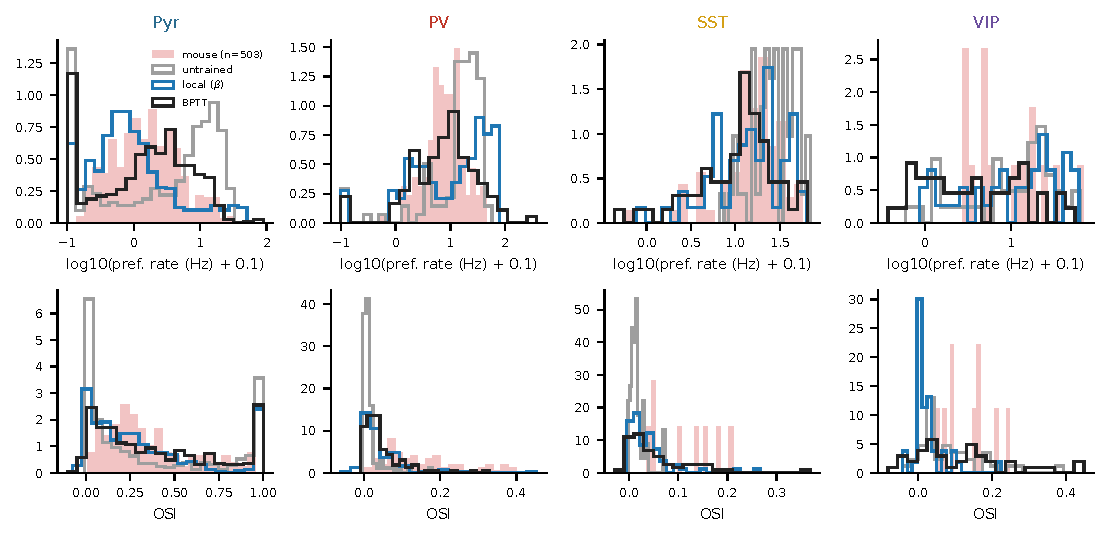
\includegraphics[width=\textwidth]{figures/fig2_tuning.pdf}
\caption{\textbf{Tuning distributions after data-matching training} (one confirmation network).
Shaded: mouse V1 Neuropixels units; lines: model cells of the same type before training and after
local or BPTT training. Top: preferred-direction rate; bottom: OSI of responsive cells.}
\label{fig:tuning}
\end{figure}

\subsection{Reliability-corrected RSA does not depend on the learning rule}
The preregistered primary endpoint is Spearman RSA between model and mouse natural-scene RDMs,
corrected for the reliability of both. It was essentially the same for every condition: 0.38 for
untrained networks, and between 0.36 and 0.39 for every trained network under both objectives
(Fig.~\ref{fig:geometry}a,g). No contrast approached significance; the largest was local vs no
$\beta$ on data matching, $-0.028$, $p=0.10$. Local vs BPTT differed by $-0.005$ [$-0.033$, $0.026$]
(data matching) and $+0.003$ [$-0.001$, $0.008$] (change detection). Together with the untrained
value, this shows that the image-similarity structure the models share with mouse V1 is set by the
fixed front end and the fitted cells, not by how the recurrent synapses were trained.

\begin{figure}[t]\centering
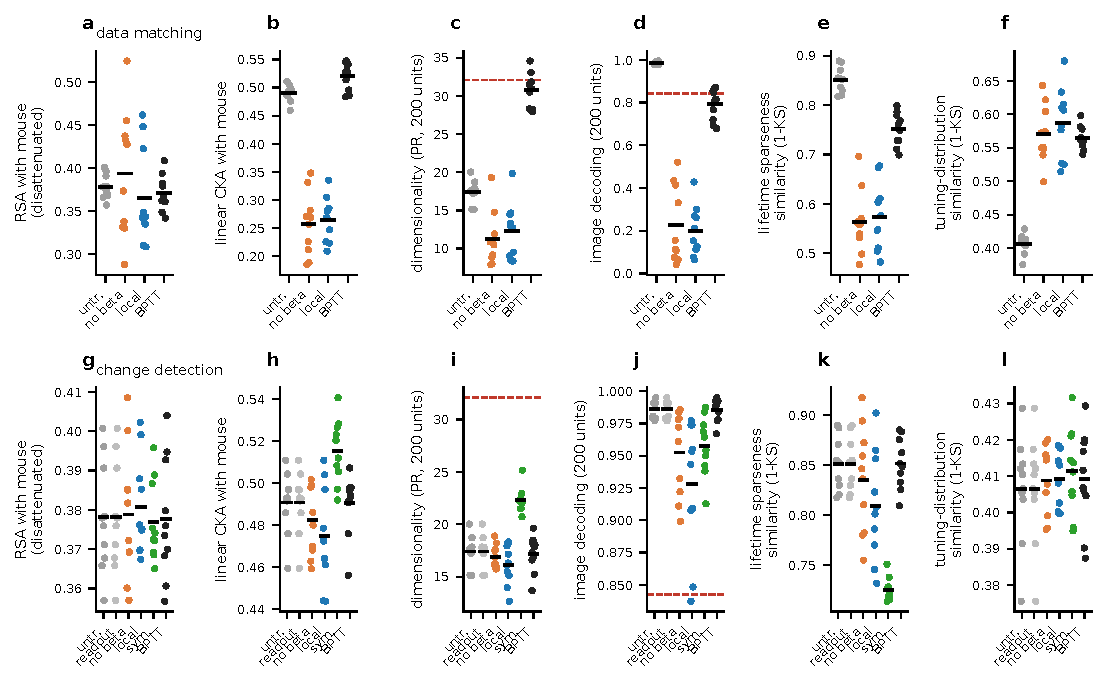
\includegraphics[width=\textwidth]{figures/fig3_geometry.pdf}
\caption{\textbf{Population geometry for 118 held-out natural scenes, compared with mouse V1.}
Each dot is one network (10 per condition); bars show means; red dashed lines show the mouse value.
(a,g) Reliability-corrected RSA (primary endpoint). (b,h) Linear CKA. (c,i) Participation ratio,
200 units. (d,j) Single-repeat image decoding, 200 units. (e,k) Lifetime-sparseness similarity.
(f,l) Mean tuning-distribution similarity. Top: data matching; bottom: change detection.}
\label{fig:geometry}
\end{figure}

\subsection{Data matching: the local rule overshoots into an image-degraded regime}
Under data matching, the secondary measures separated the rules sharply, in the same direction in
all 10 paired networks (Fig.~\ref{fig:geometry}b--e). Each of these contrasts has unadjusted
$p=0.002$, the minimum for 10 pairs. After Holm correction over the full secondary family
($\sim$40 tests) the adjusted value is $p=0.078$.

Compared with BPTT, local-trained networks had:
\begin{itemize}
\item raw RSA with the mouse 0.13 vs 0.32;
\item CKA 0.26 vs 0.52;
\item lower dimensionality: participation ratio 12 vs 31, against 32 in the mouse;
\item much poorer image decoding: 20\% vs 79\%, against 84\% in the mouse;
\item less mouse-like lifetime sparseness: similarity 0.57 vs 0.75.
\end{itemize}
Their natural-scene RDMs were also unreliable across repeats (0.14 vs 0.77). This is why the
reliability-corrected RSA was unchanged while the raw RSA fell.

The cause is visible in the circuit. On average the local rule multiplied the recurrent
magnitudes by a relative change of 87, against 2.5 for BPTT. It also drove PV cells to 43\,Hz
during natural scenes (BPTT 8\,Hz). Removing $\beta$ from the eligibility trace made no detectable
difference to any geometry measure.

\paragraph{At matched performance the rules agree.} Representations along training were related to
the data loss at each checkpoint (Fig.~\ref{fig:traj}a,b). At equal loss the local and BPTT
trajectories coincide. At the loss BPTT reached at its best ($\approx$1.5), local networks (step 200,
loss 1.39) had RSA 0.34 and CKA 0.54, the same as BPTT (0.31--0.34 and 0.51--0.54). The local
networks' geometry collapsed only after they continued past that point, fitting the
grating and gray statistics more closely than BPTT ever did. The divergence is therefore a
property of the solutions the local rule can reach, not a signature of the rule at matched
performance.

\begin{figure}[t]\centering
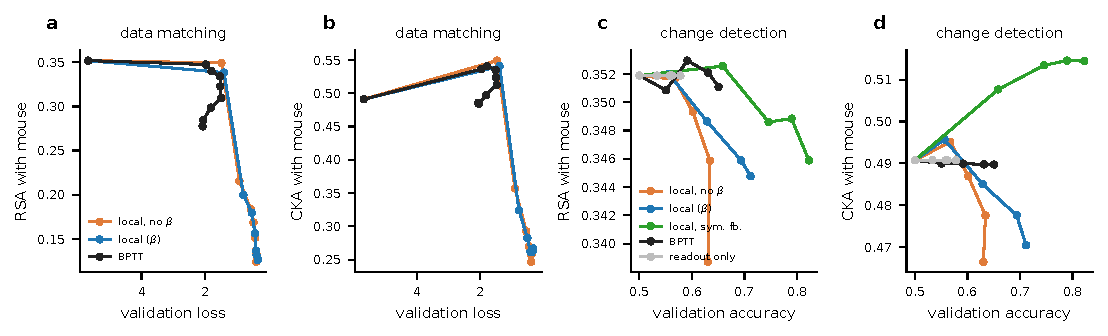
\includegraphics[width=\textwidth]{figures/fig4_trajectory.pdf}
\caption{\textbf{Geometry along training.} Mean RSA (raw) and CKA with mouse V1 at each saved
checkpoint, plotted against that checkpoint's validation value (10 networks per rule). (a,b) Data
matching (loss decreases to the right). (c,d) Change detection (accuracy).}\label{fig:traj}
\end{figure}

\subsection{Change detection: small, rule-specific changes on top of a fixed geometry}
In change detection, the local rule reached higher validation accuracy than BPTT: 0.76 vs 0.68
(readout only 0.62). Symmetric-feedback local reached 0.84. Natural-scene geometry changed little
under every rule: the correlation of each network's RDM with its own untrained RDM was 0.99
(BPTT), 0.92 (local) and 0.94 (symmetric feedback). Two consistent effects appeared, both in 10/10
networks with unadjusted $p=0.002$ (Holm-adjusted $p=0.125$):
\begin{itemize}
\item local learning slightly lowered image decoding (93\% vs 98.5\% for BPTT);
\item local learning with symmetric feedback raised dimensionality (PR 22 vs 16) and CKA with mouse
V1 (0.52 vs 0.47).
\end{itemize}

\begin{figure}[t]\centering
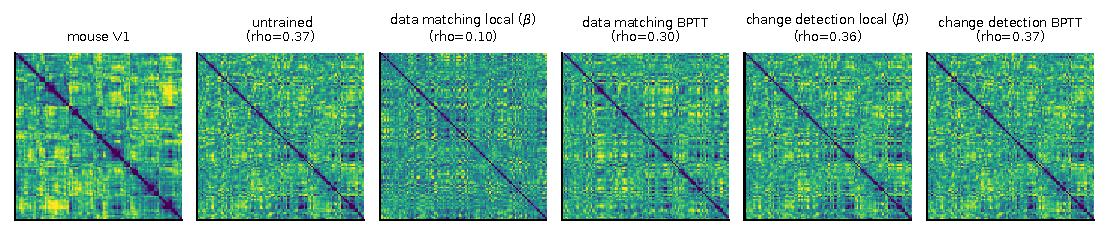
\includegraphics[width=\textwidth]{figures/fig5_rdms.pdf}
\caption{\textbf{Natural-scene RDMs} (one confirmation seed). Images are ordered by hierarchical
clustering of the mouse responses. Titles give the Spearman correlation with the mouse RDM.}
\label{fig:rdms}
\end{figure}
